\documentclass[1p]{elsarticle_modified}
%\bibliographystyle{elsarticle-num}

%\usepackage[colorlinks]{hyperref}
%\usepackage{abbrmath_seonhwa} %\Abb, \Ascr, \Acal ,\Abf, \Afrak
\usepackage{amsfonts}
\usepackage{amssymb}
\usepackage{amsmath}
\usepackage{amsthm}
\usepackage{scalefnt}
\usepackage{amsbsy}
\usepackage{kotex}
\usepackage{caption}
\usepackage{subfig}
\usepackage{color}
\usepackage{graphicx}
\usepackage{xcolor} %% white, black, red, green, blue, cyan, magenta, yellow
\usepackage{float}
\usepackage{setspace}
\usepackage{hyperref}

\usepackage{tikz}
\usetikzlibrary{arrows}

\usepackage{multirow}
\usepackage{array} % fixed length table
\usepackage{hhline}

%%%%%%%%%%%%%%%%%%%%%
\makeatletter
\renewcommand*\env@matrix[1][\arraystretch]{%
	\edef\arraystretch{#1}%
	\hskip -\arraycolsep
	\let\@ifnextchar\new@ifnextchar
	\array{*\c@MaxMatrixCols c}}
\makeatother %https://tex.stackexchange.com/questions/14071/how-can-i-increase-the-line-spacing-in-a-matrix
%%%%%%%%%%%%%%%

\usepackage[normalem]{ulem}

\newcommand{\msout}[1]{\ifmmode\text{\sout{\ensuremath{#1}}}\else\sout{#1}\fi}
%SOURCE: \msout is \stkout macro in https://tex.stackexchange.com/questions/20609/strikeout-in-math-mode

\newcommand{\cancel}[1]{
	\ifmmode
	{\color{red}\msout{#1}}
	\else
	{\color{red}\sout{#1}}
	\fi
}

\newcommand{\add}[1]{
	{\color{blue}\uwave{#1}}
}

\newcommand{\replace}[2]{
	\ifmmode
	{\color{red}\msout{#1}}{\color{blue}\uwave{#2}}
	\else
	{\color{red}\sout{#1}}{\color{blue}\uwave{#2}}
	\fi
}

\newcommand{\Sol}{\mathcal{S}} %segment
\newcommand{\D}{D} %diagram
\newcommand{\A}{\mathcal{A}} %arc


%%%%%%%%%%%%%%%%%%%%%%%%%%%%%5 test

\def\sl{\operatorname{\textup{SL}}(2,\Cbb)}
\def\psl{\operatorname{\textup{PSL}}(2,\Cbb)}
\def\quan{\mkern 1mu \triangleright \mkern 1mu}

\theoremstyle{definition}
\newtheorem{thm}{Theorem}[section]
\newtheorem{prop}[thm]{Proposition}
\newtheorem{lem}[thm]{Lemma}
\newtheorem{ques}[thm]{Question}
\newtheorem{cor}[thm]{Corollary}
\newtheorem{defn}[thm]{Definition}
\newtheorem{exam}[thm]{Example}
\newtheorem{rmk}[thm]{Remark}
\newtheorem{alg}[thm]{Algorithm}

\newcommand{\I}{\sqrt{-1}}
\begin{document}

%\begin{frontmatter}
%
%\title{Boundary parabolic representations of knots up to 8 crossings}
%
%%% Group authors per affiliation:
%\author{Yunhi Cho} 
%\address{Department of Mathematics, University of Seoul, Seoul, Korea}
%\ead{yhcho@uos.ac.kr}
%
%
%\author{Seonhwa Kim} %\fnref{s_kim}}
%\address{Center for Geometry and Physics, Institute for Basic Science, Pohang, 37673, Korea}
%\ead{ryeona17@ibs.re.kr}
%
%\author{Hyuk Kim}
%\address{Department of Mathematical Sciences, Seoul National University, Seoul 08826, Korea}
%\ead{hyukkim@snu.ac.kr}
%
%\author{Seokbeom Yoon}
%\address{Department of Mathematical Sciences, Seoul National University, Seoul, 08826,  Korea}
%\ead{sbyoon15@snu.ac.kr}
%
%\begin{abstract}
%We find all boundary parabolic representation of knots up to 8 crossings.
%
%\end{abstract}
%\begin{keyword}
%    \MSC[2010] 57M25 
%\end{keyword}
%
%\end{frontmatter}

%\linenumbers
%\tableofcontents
%
\newcommand\colored[1]{\textcolor{white}{\rule[-0.35ex]{0.8em}{1.4ex}}\kern-0.8em\color{red} #1}%
%\newcommand\colored[1]{\textcolor{white}{ #1}\kern-2.17ex	\textcolor{white}{ #1}\kern-1.81ex	\textcolor{white}{ #1}\kern-2.15ex\color{red}#1	}

{\Large $\underline{12a_{1142}~(K12a_{1142})}$}

\setlength{\tabcolsep}{10pt}
\renewcommand{\arraystretch}{1.6}
\vspace{1cm}\begin{tabular}{m{100pt}>{\centering\arraybackslash}m{274pt}}
\multirow{5}{120pt}{
	\centering
	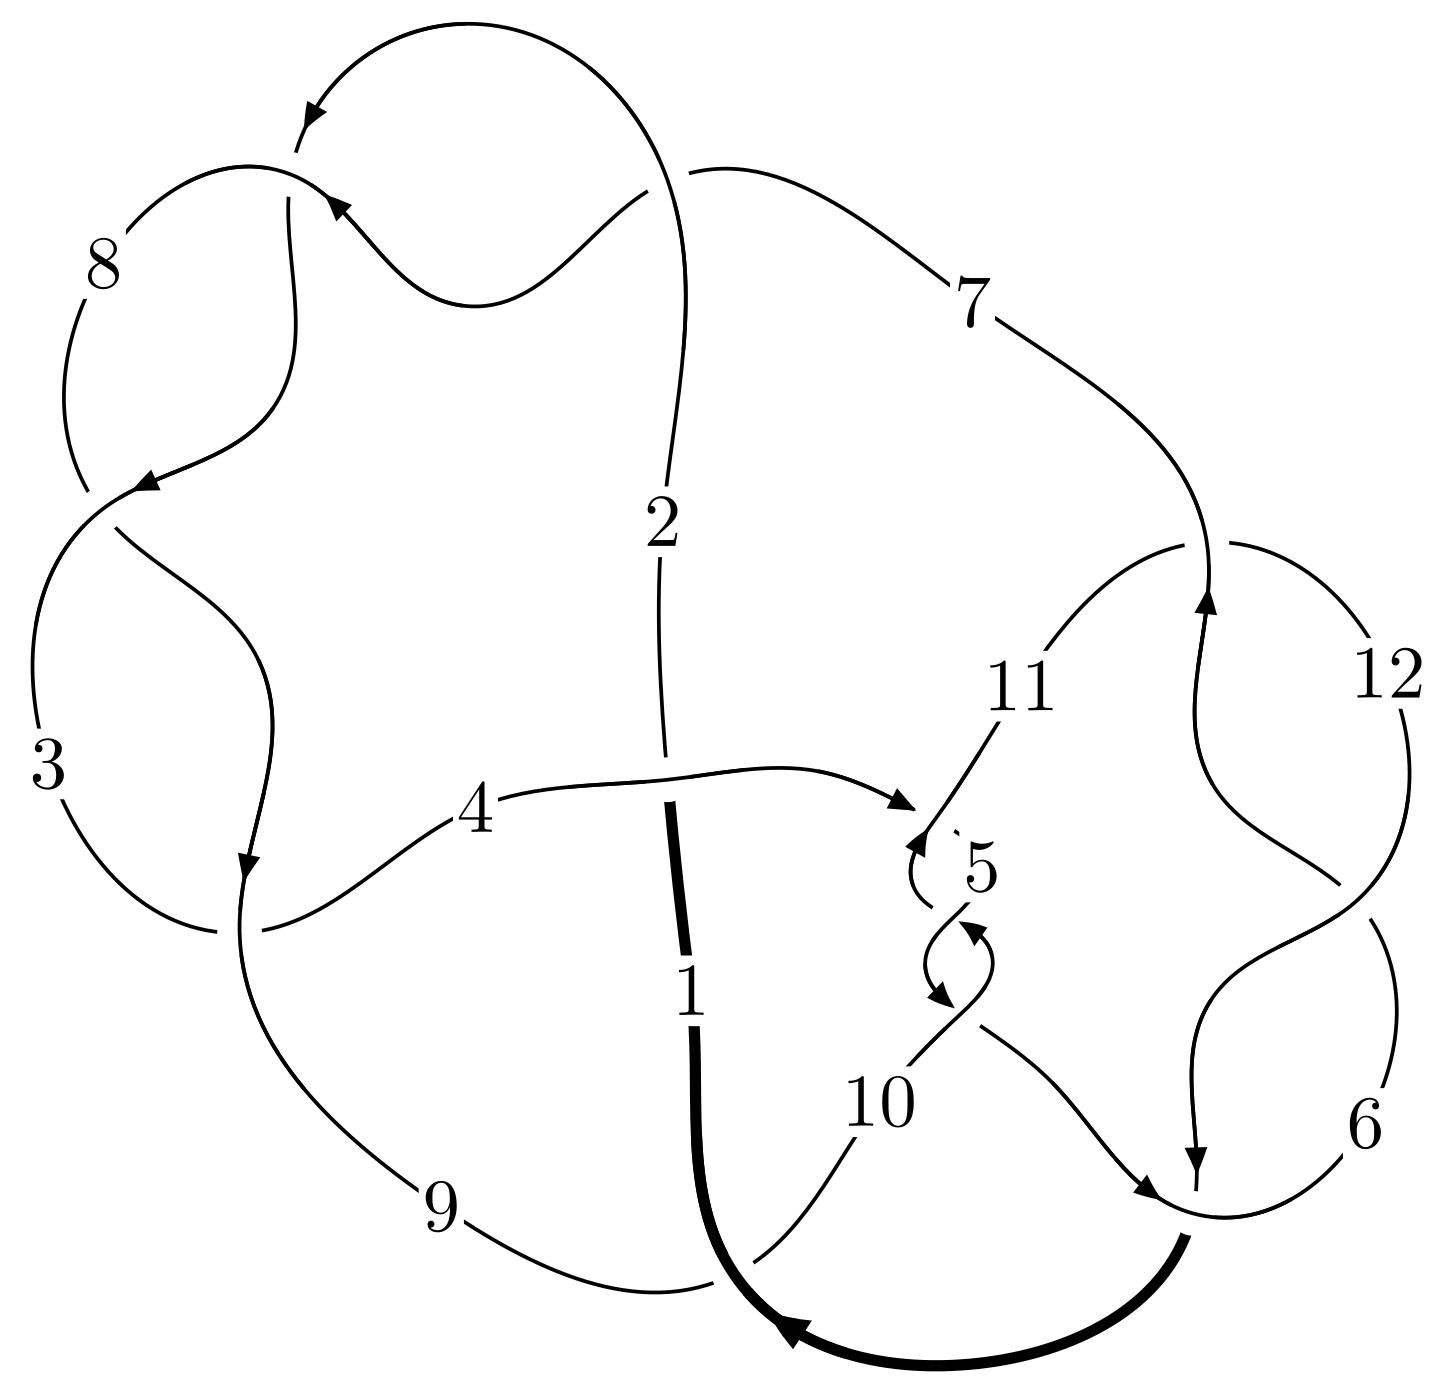
\includegraphics[width=112pt]{../../../GIT/diagram.site/Diagrams/png/1943_12a_1142.png}\\
\ \ \ A knot diagram\footnotemark}&
\allowdisplaybreaks
\textbf{Linearized knot diagam} \\
\cline{2-2}
 &
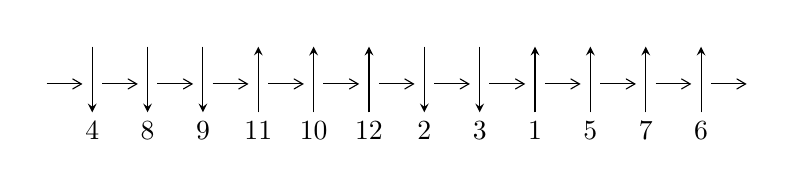
\begin{tikzpicture}[x=20pt, y=17pt]
	% nodes
	\node (C0) at (0, 0) {};
	\node (C1) at (1, 0) {};
	\node (C1U) at (1, +1) {};
	\node (C1D) at (1, -1) {4};

	\node (C2) at (2, 0) {};
	\node (C2U) at (2, +1) {};
	\node (C2D) at (2, -1) {8};

	\node (C3) at (3, 0) {};
	\node (C3U) at (3, +1) {};
	\node (C3D) at (3, -1) {9};

	\node (C4) at (4, 0) {};
	\node (C4U) at (4, +1) {};
	\node (C4D) at (4, -1) {11};

	\node (C5) at (5, 0) {};
	\node (C5U) at (5, +1) {};
	\node (C5D) at (5, -1) {10};

	\node (C6) at (6, 0) {};
	\node (C6U) at (6, +1) {};
	\node (C6D) at (6, -1) {12};

	\node (C7) at (7, 0) {};
	\node (C7U) at (7, +1) {};
	\node (C7D) at (7, -1) {2};

	\node (C8) at (8, 0) {};
	\node (C8U) at (8, +1) {};
	\node (C8D) at (8, -1) {3};

	\node (C9) at (9, 0) {};
	\node (C9U) at (9, +1) {};
	\node (C9D) at (9, -1) {1};

	\node (C10) at (10, 0) {};
	\node (C10U) at (10, +1) {};
	\node (C10D) at (10, -1) {5};

	\node (C11) at (11, 0) {};
	\node (C11U) at (11, +1) {};
	\node (C11D) at (11, -1) {7};

	\node (C12) at (12, 0) {};
	\node (C12U) at (12, +1) {};
	\node (C12D) at (12, -1) {6};
	\node (C13) at (13, 0) {};

	% arrows
	\draw[->,>={angle 60}]
	(C0) edge (C1) (C1) edge (C2) (C2) edge (C3) (C3) edge (C4) (C4) edge (C5) (C5) edge (C6) (C6) edge (C7) (C7) edge (C8) (C8) edge (C9) (C9) edge (C10) (C10) edge (C11) (C11) edge (C12) (C12) edge (C13) ;	\draw[->,>=stealth]
	(C1U) edge (C1D) (C2U) edge (C2D) (C3U) edge (C3D) (C4D) edge (C4U) (C5D) edge (C5U) (C6D) edge (C6U) (C7U) edge (C7D) (C8U) edge (C8D) (C9D) edge (C9U) (C10D) edge (C10U) (C11D) edge (C11U) (C12D) edge (C12U) ;
	\end{tikzpicture} \\
\hhline{~~} \\& 
\textbf{Solving Sequence} \\ \cline{2-2} 
 &
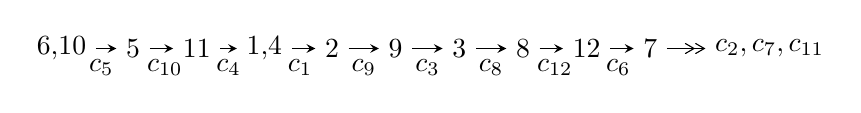
\begin{tikzpicture}[x=23pt, y=7pt]
	% node
	\node (A0) at (-1/8, 0) {6,10};
	\node (A1) at (1, 0) {5};
	\node (A2) at (2, 0) {11};
	\node (A3) at (49/16, 0) {1,4};
	\node (A4) at (33/8, 0) {2};
	\node (A5) at (41/8, 0) {9};
	\node (A6) at (49/8, 0) {3};
	\node (A7) at (57/8, 0) {8};
	\node (A8) at (65/8, 0) {12};
	\node (A9) at (73/8, 0) {7};
	\node (C1) at (1/2, -1) {$c_{5}$};
	\node (C2) at (3/2, -1) {$c_{10}$};
	\node (C3) at (5/2, -1) {$c_{4}$};
	\node (C4) at (29/8, -1) {$c_{1}$};
	\node (C5) at (37/8, -1) {$c_{9}$};
	\node (C6) at (45/8, -1) {$c_{3}$};
	\node (C7) at (53/8, -1) {$c_{8}$};
	\node (C8) at (61/8, -1) {$c_{12}$};
	\node (C9) at (69/8, -1) {$c_{6}$};
	\node (A10) at (11, 0) {$c_{2},c_{7},c_{11}$};

	% edge
	\draw[->,>=stealth]	
	(A0) edge (A1) (A1) edge (A2) (A2) edge (A3) (A3) edge (A4) (A4) edge (A5) (A5) edge (A6) (A6) edge (A7) (A7) edge (A8) (A8) edge (A9) ;
	\draw[->>,>={angle 60}]	
	(A9) edge (A10);
\end{tikzpicture} \\ 

\end{tabular} \\

\footnotetext{
The image of knot diagram is generated by the software ``\textbf{Draw programme}" developed by Andrew Bartholomew(\url{http://www.layer8.co.uk/maths/draw/index.htm\#Running-draw}), where we modified some parts for our purpose(\url{https://github.com/CATsTAILs/LinksPainter}).
}\phantom \\ \newline 
\centering \textbf{Ideals for irreducible components\footnotemark of $X_{\text{par}}$} 
 
\begin{align*}
I^u_{1}&=\langle 
b- u,\;- u^{24}- u^{23}+\cdots+16 a+1,\;u^{25}+16 u^{23}+\cdots- u-1\rangle \\
I^u_{2}&=\langle 
31265112052 u^{31}-16257768219 u^{30}+\cdots+84752307686 b-8778222360,\\
\phantom{I^u_{2}}&\phantom{= \langle  }-11111041791 u^{31}+26118385624 u^{30}+\cdots+84752307686 a+287854854541,\\
\phantom{I^u_{2}}&\phantom{= \langle  }u^{32}- u^{31}+\cdots-7 u+2\rangle \\
I^u_{3}&=\langle 
b+u,\;a^4- a^3+a^2+1,\;u^2+1\rangle \\
\\
\end{align*}
\raggedright * 3 irreducible components of $\dim_{\mathbb{C}}=0$, with total 65 representations.\\
\footnotetext{All coefficients of polynomials are rational numbers. But the coefficients are sometimes approximated in decimal forms when there is not enough margin.}
\newpage
\renewcommand{\arraystretch}{1}
\centering \section*{I. $I^u_{1}= \langle b- u,\;- u^{24}- u^{23}+\cdots+16 a+1,\;u^{25}+16 u^{23}+\cdots- u-1 \rangle$}
\flushleft \textbf{(i) Arc colorings}\\
\begin{tabular}{m{7pt} m{180pt} m{7pt} m{180pt} }
\flushright $a_{6}=$&$\begin{pmatrix}1\\0\end{pmatrix}$ \\
\flushright $a_{10}=$&$\begin{pmatrix}0\\u\end{pmatrix}$ \\
\flushright $a_{5}=$&$\begin{pmatrix}1\\u^2\end{pmatrix}$ \\
\flushright $a_{11}=$&$\begin{pmatrix}u\\u^3+u\end{pmatrix}$ \\
\flushright $a_{1}=$&$\begin{pmatrix}\frac{1}{16} u^{24}+\frac{1}{16} u^{23}+\cdots+\frac{23}{8} u-\frac{1}{16}\\u\end{pmatrix}$ \\
\flushright $a_{4}=$&$\begin{pmatrix}u^2+1\\u^4+2 u^2\end{pmatrix}$ \\
\flushright $a_{2}=$&$\begin{pmatrix}\frac{1}{16} u^{24}+\frac{1}{16} u^{23}+\cdots+\frac{15}{8} u-\frac{1}{16}\\\frac{1}{16} u^{24}+\frac{1}{16} u^{23}+\cdots+\frac{7}{8} u-\frac{1}{16}\end{pmatrix}$ \\
\flushright $a_{9}=$&$\begin{pmatrix}\frac{1}{8} u^{24}+2 u^{22}+\cdots-\frac{3}{8} u-\frac{1}{8}\\\frac{1}{16} u^{24}+\frac{1}{16} u^{23}+\cdots+\frac{7}{8} u-\frac{1}{16}\end{pmatrix}$ \\
\flushright $a_{3}=$&$\begin{pmatrix}\frac{3}{16} u^{24}+\frac{3}{16} u^{23}+\cdots-\frac{5}{8} u-\frac{5}{16}\\-\frac{1}{4} u^{24}+\frac{3}{8} u^{23}+\cdots-\frac{1}{8} u-\frac{5}{8}\end{pmatrix}$ \\
\flushright $a_{8}=$&$\begin{pmatrix}\frac{3}{16} u^{24}-\frac{5}{16} u^{23}+\cdots+\frac{1}{8} u+\frac{23}{16}\\-\frac{1}{8} u^{23}+\frac{1}{4} u^{22}+\cdots+\frac{1}{8} u+\frac{5}{8}\end{pmatrix}$ \\
\flushright $a_{12}=$&$\begin{pmatrix}\frac{1}{16} u^{24}+\frac{1}{16} u^{23}+\cdots+\frac{15}{8} u-\frac{1}{16}\\u\end{pmatrix}$ \\
\flushright $a_{7}=$&$\begin{pmatrix}-0.0625000 u^{24}+0.0625000 u^{23}+\cdots-2.12500 u^{2}+0.937500\\- u^2\end{pmatrix}$\\&\end{tabular}
\flushleft \textbf{(ii) Obstruction class $= -1$}\\~\\
\flushleft \textbf{(iii) Cusp Shapes $= -2 u^{24}+\frac{5}{4} u^{23}+\cdots+\frac{5}{4} u-\frac{1}{2}$}\\~\\
\newpage\renewcommand{\arraystretch}{1}
\flushleft \textbf{(iv) u-Polynomials at the component}\newline \\
\begin{tabular}{m{50pt}|m{274pt}}
Crossings & \hspace{64pt}u-Polynomials at each crossing \\
\hline $$\begin{aligned}c_{1}\end{aligned}$$&$\begin{aligned}
&u^{25}-7 u^{24}+\cdots+513 u-136
\end{aligned}$\\
\hline $$\begin{aligned}c_{2},c_{3},c_{7}\\c_{8}\end{aligned}$$&$\begin{aligned}
&u^{25}+3 u^{24}+\cdots-3 u+2
\end{aligned}$\\
\hline $$\begin{aligned}c_{4},c_{5},c_{6}\\c_{10},c_{11},c_{12}\end{aligned}$$&$\begin{aligned}
&u^{25}+16 u^{23}+\cdots- u+1
\end{aligned}$\\
\hline $$\begin{aligned}c_{9}\end{aligned}$$&$\begin{aligned}
&u^{25}-15 u^{24}+\cdots+2387 u-362
\end{aligned}$\\
\hline
\end{tabular}\\~\\
\newpage\renewcommand{\arraystretch}{1}
\flushleft \textbf{(v) Riley Polynomials at the component}\newline \\
\begin{tabular}{m{50pt}|m{274pt}}
Crossings & \hspace{64pt}Riley Polynomials at each crossing \\
\hline $$\begin{aligned}c_{1}\end{aligned}$$&$\begin{aligned}
&y^{25}-5 y^{24}+\cdots-37119 y-18496
\end{aligned}$\\
\hline $$\begin{aligned}c_{2},c_{3},c_{7}\\c_{8}\end{aligned}$$&$\begin{aligned}
&y^{25}-29 y^{24}+\cdots+y-4
\end{aligned}$\\
\hline $$\begin{aligned}c_{4},c_{5},c_{6}\\c_{10},c_{11},c_{12}\end{aligned}$$&$\begin{aligned}
&y^{25}+32 y^{24}+\cdots-7 y-1
\end{aligned}$\\
\hline $$\begin{aligned}c_{9}\end{aligned}$$&$\begin{aligned}
&y^{25}+11 y^{24}+\cdots-420031 y-131044
\end{aligned}$\\
\hline
\end{tabular}\\~\\
\newpage\flushleft \textbf{(vi) Complex Volumes and Cusp Shapes}
$$\begin{array}{c|c|c}  
\text{Solutions to }I^u_{1}& \I (\text{vol} + \sqrt{-1}CS) & \text{Cusp shape}\\
 \hline 
\begin{aligned}
u &= -0.561043 + 0.437348 I \\
a &= -1.68535 + 0.72480 I \\
b &= -0.561043 + 0.437348 I\end{aligned}
 & -7.98772 - 5.54613 I & -2.08956 + 7.04826 I \\ \hline\begin{aligned}
u &= -0.561043 - 0.437348 I \\
a &= -1.68535 - 0.72480 I \\
b &= -0.561043 - 0.437348 I\end{aligned}
 & -7.98772 + 5.54613 I & -2.08956 - 7.04826 I \\ \hline\begin{aligned}
u &= \phantom{-}0.638286\phantom{ +0.000000I} \\
a &= \phantom{-}1.54532\phantom{ +0.000000I} \\
b &= \phantom{-}0.638286\phantom{ +0.000000I}\end{aligned}
 & -4.66650\phantom{ +0.000000I} & \phantom{-}2.55840\phantom{ +0.000000I} \\ \hline\begin{aligned}
u &= \phantom{-}0.521660 + 0.351950 I \\
a &= \phantom{-}1.52382 + 0.64449 I \\
b &= \phantom{-}0.521660 + 0.351950 I\end{aligned}
 & -0.34952 + 3.61361 I & \phantom{-}0.91371 - 9.39805 I \\ \hline\begin{aligned}
u &= \phantom{-}0.521660 - 0.351950 I \\
a &= \phantom{-}1.52382 - 0.64449 I \\
b &= \phantom{-}0.521660 - 0.351950 I\end{aligned}
 & -0.34952 - 3.61361 I & \phantom{-}0.91371 + 9.39805 I \\ \hline\begin{aligned}
u &= -0.200130 + 0.529662 I \\
a &= -1.05021 + 1.68712 I \\
b &= -0.200130 + 0.529662 I\end{aligned}
 & -8.41951 + 2.51161 I & -3.21376 + 1.03660 I \\ \hline\begin{aligned}
u &= -0.200130 - 0.529662 I \\
a &= -1.05021 - 1.68712 I \\
b &= -0.200130 - 0.529662 I\end{aligned}
 & -8.41951 - 2.51161 I & -3.21376 - 1.03660 I \\ \hline\begin{aligned}
u &= -0.09775 + 1.44695 I \\
a &= -0.581028 - 1.096330 I \\
b &= -0.09775 + 1.44695 I\end{aligned}
 & -13.25460 - 4.79321 I & -7.77691 + 3.39473 I \\ \hline\begin{aligned}
u &= -0.09775 - 1.44695 I \\
a &= -0.581028 + 1.096330 I \\
b &= -0.09775 - 1.44695 I\end{aligned}
 & -13.25460 + 4.79321 I & -7.77691 - 3.39473 I \\ \hline\begin{aligned}
u &= \phantom{-}0.02846 + 1.45258 I \\
a &= \phantom{-}0.171580 - 1.155960 I \\
b &= \phantom{-}0.02846 + 1.45258 I\end{aligned}
 & -6.93212 + 2.05900 I & -4.36476 - 3.38495 I\\
 \hline 
 \end{array}$$\newpage$$\begin{array}{c|c|c}  
\text{Solutions to }I^u_{1}& \I (\text{vol} + \sqrt{-1}CS) & \text{Cusp shape}\\
 \hline 
\begin{aligned}
u &= \phantom{-}0.02846 - 1.45258 I \\
a &= \phantom{-}0.171580 + 1.155960 I \\
b &= \phantom{-}0.02846 - 1.45258 I\end{aligned}
 & -6.93212 - 2.05900 I & -4.36476 + 3.38495 I \\ \hline\begin{aligned}
u &= -0.464935 + 0.201716 I \\
a &= -1.289760 + 0.413307 I \\
b &= -0.464935 + 0.201716 I\end{aligned}
 & \phantom{-}0.912372 - 0.622752 I & \phantom{-}7.19624 + 2.63067 I \\ \hline\begin{aligned}
u &= -0.464935 - 0.201716 I \\
a &= -1.289760 - 0.413307 I \\
b &= -0.464935 - 0.201716 I\end{aligned}
 & \phantom{-}0.912372 + 0.622752 I & \phantom{-}7.19624 - 2.63067 I \\ \hline\begin{aligned}
u &= \phantom{-}0.166735 + 0.405495 I \\
a &= \phantom{-}0.68732 + 1.26329 I \\
b &= \phantom{-}0.166735 + 0.405495 I\end{aligned}
 & -1.020640 - 0.969548 I & -2.52284 + 1.35231 I \\ \hline\begin{aligned}
u &= \phantom{-}0.166735 - 0.405495 I \\
a &= \phantom{-}0.68732 - 1.26329 I \\
b &= \phantom{-}0.166735 - 0.405495 I\end{aligned}
 & -1.020640 + 0.969548 I & -2.52284 - 1.35231 I \\ \hline\begin{aligned}
u &= \phantom{-}0.27079 + 1.54625 I \\
a &= \phantom{-}1.040560 - 0.311629 I \\
b &= \phantom{-}0.27079 + 1.54625 I\end{aligned}
 & -11.13940 + 6.44106 I & -3.32238 - 2.71115 I \\ \hline\begin{aligned}
u &= \phantom{-}0.27079 - 1.54625 I \\
a &= \phantom{-}1.040560 + 0.311629 I \\
b &= \phantom{-}0.27079 - 1.54625 I\end{aligned}
 & -11.13940 - 6.44106 I & -3.32238 + 2.71115 I \\ \hline\begin{aligned}
u &= -0.31312 + 1.55281 I \\
a &= -1.136180 - 0.202662 I \\
b &= -0.31312 + 1.55281 I\end{aligned}
 & -13.0092 - 10.4518 I & -6.37304 + 7.21331 I \\ \hline\begin{aligned}
u &= -0.31312 - 1.55281 I \\
a &= -1.136180 + 0.202662 I \\
b &= -0.31312 - 1.55281 I\end{aligned}
 & -13.0092 + 10.4518 I & -6.37304 - 7.21331 I \\ \hline\begin{aligned}
u &= -0.21804 + 1.58247 I \\
a &= -0.814184 - 0.307816 I \\
b &= -0.21804 + 1.58247 I\end{aligned}
 & -14.4736 - 3.0731 I & -8.36964 + 0. I\phantom{ +0.000000I}\\
 \hline 
 \end{array}$$\newpage$$\begin{array}{c|c|c}  
\text{Solutions to }I^u_{1}& \I (\text{vol} + \sqrt{-1}CS) & \text{Cusp shape}\\
 \hline 
\begin{aligned}
u &= -0.21804 - 1.58247 I \\
a &= -0.814184 + 0.307816 I \\
b &= -0.21804 - 1.58247 I\end{aligned}
 & -14.4736 + 3.0731 I & -8.36964 + 0. I\phantom{ +0.000000I} \\ \hline\begin{aligned}
u &= \phantom{-}0.34476 + 1.56544 I \\
a &= \phantom{-}1.182290 - 0.106671 I \\
b &= \phantom{-}0.34476 + 1.56544 I\end{aligned}
 & \phantom{-}18.3511 + 13.0389 I & -8.43014 - 5.93322 I \\ \hline\begin{aligned}
u &= \phantom{-}0.34476 - 1.56544 I \\
a &= \phantom{-}1.182290 + 0.106671 I \\
b &= \phantom{-}0.34476 - 1.56544 I\end{aligned}
 & \phantom{-}18.3511 - 13.0389 I & -8.43014 + 5.93322 I \\ \hline\begin{aligned}
u &= \phantom{-}0.20347 + 1.64400 I \\
a &= \phantom{-}0.678475 - 0.143846 I \\
b &= \phantom{-}0.20347 + 1.64400 I\end{aligned}
 & \phantom{-}16.0652 + 1.5629 I & -9.92611 - 0.62064 I \\ \hline\begin{aligned}
u &= \phantom{-}0.20347 - 1.64400 I \\
a &= \phantom{-}0.678475 + 0.143846 I \\
b &= \phantom{-}0.20347 - 1.64400 I\end{aligned}
 & \phantom{-}16.0652 - 1.5629 I & -9.92611 + 0.62064 I\\
 \hline 
 \end{array}$$\newpage\newpage\renewcommand{\arraystretch}{1}
\centering \section*{II. $I^u_{2}= \langle 3.13\times10^{10} u^{31}-1.63\times10^{10} u^{30}+\cdots+8.48\times10^{10} b-8.78\times10^{9},\;-1.11\times10^{10} u^{31}+2.61\times10^{10} u^{30}+\cdots+8.48\times10^{10} a+2.88\times10^{11},\;u^{32}- u^{31}+\cdots-7 u+2 \rangle$}
\flushleft \textbf{(i) Arc colorings}\\
\begin{tabular}{m{7pt} m{180pt} m{7pt} m{180pt} }
\flushright $a_{6}=$&$\begin{pmatrix}1\\0\end{pmatrix}$ \\
\flushright $a_{10}=$&$\begin{pmatrix}0\\u\end{pmatrix}$ \\
\flushright $a_{5}=$&$\begin{pmatrix}1\\u^2\end{pmatrix}$ \\
\flushright $a_{11}=$&$\begin{pmatrix}u\\u^3+u\end{pmatrix}$ \\
\flushright $a_{1}=$&$\begin{pmatrix}0.131100 u^{31}-0.308173 u^{30}+\cdots+2.64660 u-3.39642\\-0.368900 u^{31}+0.191827 u^{30}+\cdots-2.85340 u+0.103575\end{pmatrix}$ \\
\flushright $a_{4}=$&$\begin{pmatrix}u^2+1\\u^4+2 u^2\end{pmatrix}$ \\
\flushright $a_{2}=$&$\begin{pmatrix}0.257094 u^{31}-0.416002 u^{30}+\cdots+3.69092 u-3.68254\\-0.652251 u^{31}+0.451316 u^{30}+\cdots-4.12999 u+0.211450\end{pmatrix}$ \\
\flushright $a_{9}=$&$\begin{pmatrix}0.0315636 u^{31}-0.0452649 u^{30}+\cdots+0.291482 u-2.93870\\-0.0995366 u^{31}+0.262908 u^{30}+\cdots-1.35511 u+0.457721\end{pmatrix}$ \\
\flushright $a_{3}=$&$\begin{pmatrix}-0.458023 u^{31}+0.342355 u^{30}+\cdots-6.00927 u+2.47313\\0.0217054 u^{31}-0.180440 u^{30}+\cdots+4.15577 u-0.559030\end{pmatrix}$ \\
\flushright $a_{8}=$&$\begin{pmatrix}0.220688 u^{31}-0.0368277 u^{30}+\cdots-0.676663 u-2.74045\\0.269259 u^{31}+0.0522139 u^{30}+\cdots-2.98024 u+1.30099\end{pmatrix}$ \\
\flushright $a_{12}=$&$\begin{pmatrix}\frac{1}{2} u^{31}-\frac{1}{2} u^{30}+\cdots+\frac{11}{2} u-\frac{7}{2}\\-0.368900 u^{31}+0.191827 u^{30}+\cdots-2.85340 u+0.103575\end{pmatrix}$ \\
\flushright $a_{7}=$&$\begin{pmatrix}-0.0517875 u^{31}-0.317112 u^{30}+\cdots-10.4579 u-1.49089\\-0.177073 u^{31}+0.446436 u^{30}+\cdots-2.47872 u+1.73780\end{pmatrix}$\\&\end{tabular}
\flushleft \textbf{(ii) Obstruction class $= -1$}\\~\\
\flushleft \textbf{(iii) Cusp Shapes $= -\frac{27044210812}{42376153843} u^{31}-\frac{8739385902}{42376153843} u^{30}+\cdots-\frac{295063087682}{42376153843} u+\frac{92212569266}{42376153843}$}\\~\\
\newpage\renewcommand{\arraystretch}{1}
\flushleft \textbf{(iv) u-Polynomials at the component}\newline \\
\begin{tabular}{m{50pt}|m{274pt}}
Crossings & \hspace{64pt}u-Polynomials at each crossing \\
\hline $$\begin{aligned}c_{1}\end{aligned}$$&$\begin{aligned}
&(u^{16}-5 u^{15}+\cdots+8 u-7)^{2}
\end{aligned}$\\
\hline $$\begin{aligned}c_{2},c_{3},c_{7}\\c_{8}\end{aligned}$$&$\begin{aligned}
&(u^{16}- u^{15}+\cdots+2 u^2-1)^{2}
\end{aligned}$\\
\hline $$\begin{aligned}c_{4},c_{5},c_{6}\\c_{10},c_{11},c_{12}\end{aligned}$$&$\begin{aligned}
&u^{32}+u^{31}+\cdots+7 u+2
\end{aligned}$\\
\hline $$\begin{aligned}c_{9}\end{aligned}$$&$\begin{aligned}
&(u^{16}+5 u^{15}+\cdots-4 u+1)^{2}
\end{aligned}$\\
\hline
\end{tabular}\\~\\
\newpage\renewcommand{\arraystretch}{1}
\flushleft \textbf{(v) Riley Polynomials at the component}\newline \\
\begin{tabular}{m{50pt}|m{274pt}}
Crossings & \hspace{64pt}Riley Polynomials at each crossing \\
\hline $$\begin{aligned}c_{1}\end{aligned}$$&$\begin{aligned}
&(y^{16}-7 y^{15}+\cdots-344 y+49)^{2}
\end{aligned}$\\
\hline $$\begin{aligned}c_{2},c_{3},c_{7}\\c_{8}\end{aligned}$$&$\begin{aligned}
&(y^{16}-19 y^{15}+\cdots-4 y+1)^{2}
\end{aligned}$\\
\hline $$\begin{aligned}c_{4},c_{5},c_{6}\\c_{10},c_{11},c_{12}\end{aligned}$$&$\begin{aligned}
&y^{32}+27 y^{31}+\cdots-5 y+4
\end{aligned}$\\
\hline $$\begin{aligned}c_{9}\end{aligned}$$&$\begin{aligned}
&(y^{16}+13 y^{15}+\cdots-48 y+1)^{2}
\end{aligned}$\\
\hline
\end{tabular}\\~\\
\newpage\flushleft \textbf{(vi) Complex Volumes and Cusp Shapes}
$$\begin{array}{c|c|c}  
\text{Solutions to }I^u_{2}& \I (\text{vol} + \sqrt{-1}CS) & \text{Cusp shape}\\
 \hline 
\begin{aligned}
u &= -0.880391 + 0.506625 I \\
a &= \phantom{-}1.017130 - 0.972732 I \\
b &= \phantom{-}0.16383 - 1.46376 I\end{aligned}
 & -6.29225 - 6.07197 I & -4.61575 + 7.02814 I \\ \hline\begin{aligned}
u &= -0.880391 - 0.506625 I \\
a &= \phantom{-}1.017130 + 0.972732 I \\
b &= \phantom{-}0.16383 + 1.46376 I\end{aligned}
 & -6.29225 + 6.07197 I & -4.61575 - 7.02814 I \\ \hline\begin{aligned}
u &= -0.774157 + 0.692338 I \\
a &= \phantom{-}0.741176 - 0.809846 I \\
b &= \phantom{-}0.02347 - 1.45170 I\end{aligned}
 & -6.89084 + 0.48968 I & -6.35607 - 1.43137 I \\ \hline\begin{aligned}
u &= -0.774157 - 0.692338 I \\
a &= \phantom{-}0.741176 + 0.809846 I \\
b &= \phantom{-}0.02347 + 1.45170 I\end{aligned}
 & -6.89084 - 0.48968 I & -6.35607 + 1.43137 I \\ \hline\begin{aligned}
u &= \phantom{-}0.777840 + 0.542265 I \\
a &= -0.977635 - 0.812403 I \\
b &= -0.11249 - 1.41553 I\end{aligned}
 & -4.30716 + 2.57669 I & -0.69244 - 2.71681 I \\ \hline\begin{aligned}
u &= \phantom{-}0.777840 - 0.542265 I \\
a &= -0.977635 + 0.812403 I \\
b &= -0.11249 + 1.41553 I\end{aligned}
 & -4.30716 - 2.57669 I & -0.69244 + 2.71681 I \\ \hline\begin{aligned}
u &= \phantom{-}0.192406 + 1.054070 I \\
a &= \phantom{-}0.0248167 - 0.1359550 I \\
b &= \phantom{-}0.192406 - 1.054070 I\end{aligned}
 & -4.05396\phantom{ +0.000000I} & -9.09362 + 0. I\phantom{ +0.000000I} \\ \hline\begin{aligned}
u &= \phantom{-}0.192406 - 1.054070 I \\
a &= \phantom{-}0.0248167 + 0.1359550 I \\
b &= \phantom{-}0.192406 + 1.054070 I\end{aligned}
 & -4.05396\phantom{ +0.000000I} & -9.09362 + 0. I\phantom{ +0.000000I} \\ \hline\begin{aligned}
u &= \phantom{-}0.949812 + 0.504302 I \\
a &= -1.00934 - 1.06834 I \\
b &= -0.18803 - 1.50441 I\end{aligned}
 & -14.4043 + 8.2886 I & -6.57708 - 5.27135 I \\ \hline\begin{aligned}
u &= \phantom{-}0.949812 - 0.504302 I \\
a &= -1.00934 + 1.06834 I \\
b &= -0.18803 + 1.50441 I\end{aligned}
 & -14.4043 - 8.2886 I & -6.57708 + 5.27135 I\\
 \hline 
 \end{array}$$\newpage$$\begin{array}{c|c|c}  
\text{Solutions to }I^u_{2}& \I (\text{vol} + \sqrt{-1}CS) & \text{Cusp shape}\\
 \hline 
\begin{aligned}
u &= -0.060795 + 1.080160 I \\
a &= \phantom{-}0.211903 + 0.762923 I \\
b &= \phantom{-}0.159960 - 0.159944 I\end{aligned}
 & -1.40282 - 1.52971 I & \phantom{-}2.72737 + 5.08772 I \\ \hline\begin{aligned}
u &= -0.060795 - 1.080160 I \\
a &= \phantom{-}0.211903 - 0.762923 I \\
b &= \phantom{-}0.159960 + 0.159944 I\end{aligned}
 & -1.40282 + 1.52971 I & \phantom{-}2.72737 - 5.08772 I \\ \hline\begin{aligned}
u &= \phantom{-}0.195301 + 1.117820 I \\
a &= -0.601834 + 0.773671 I \\
b &= -0.450162 - 0.094431 I\end{aligned}
 & -7.98944 + 3.12434 I & -1.94060 - 3.66013 I \\ \hline\begin{aligned}
u &= \phantom{-}0.195301 - 1.117820 I \\
a &= -0.601834 - 0.773671 I \\
b &= -0.450162 + 0.094431 I\end{aligned}
 & -7.98944 - 3.12434 I & -1.94060 + 3.66013 I \\ \hline\begin{aligned}
u &= \phantom{-}0.840396 + 0.765707 I \\
a &= -0.642609 - 0.918714 I \\
b &= \phantom{-}0.00756 - 1.51110 I\end{aligned}
 & -15.1904 - 2.2836 I & -7.92472 + 0.30826 I \\ \hline\begin{aligned}
u &= \phantom{-}0.840396 - 0.765707 I \\
a &= -0.642609 + 0.918714 I \\
b &= \phantom{-}0.00756 + 1.51110 I\end{aligned}
 & -15.1904 + 2.2836 I & -7.92472 - 0.30826 I \\ \hline\begin{aligned}
u &= -0.344556 + 1.164540 I \\
a &= -0.110939 - 0.374956 I \\
b &= -0.344556 - 1.164540 I\end{aligned}
 & -11.2964\phantom{ +0.000000I} & -8.14780 + 0. I\phantom{ +0.000000I} \\ \hline\begin{aligned}
u &= -0.344556 - 1.164540 I \\
a &= -0.110939 + 0.374956 I \\
b &= -0.344556 + 1.164540 I\end{aligned}
 & -11.2964\phantom{ +0.000000I} & -8.14780 + 0. I\phantom{ +0.000000I} \\ \hline\begin{aligned}
u &= -0.11249 + 1.41553 I \\
a &= \phantom{-}0.833628 + 0.159750 I \\
b &= \phantom{-}0.777840 - 0.542265 I\end{aligned}
 & -4.30716 - 2.57669 I & -0.69244 + 2.71681 I \\ \hline\begin{aligned}
u &= -0.11249 - 1.41553 I \\
a &= \phantom{-}0.833628 - 0.159750 I \\
b &= \phantom{-}0.777840 + 0.542265 I\end{aligned}
 & -4.30716 + 2.57669 I & -0.69244 - 2.71681 I\\
 \hline 
 \end{array}$$\newpage$$\begin{array}{c|c|c}  
\text{Solutions to }I^u_{2}& \I (\text{vol} + \sqrt{-1}CS) & \text{Cusp shape}\\
 \hline 
\begin{aligned}
u &= \phantom{-}0.02347 + 1.45170 I \\
a &= -0.785289 - 0.003672 I \\
b &= -0.774157 - 0.692338 I\end{aligned}
 & -6.89084 - 0.48968 I & -6.35607 + 1.43137 I \\ \hline\begin{aligned}
u &= \phantom{-}0.02347 - 1.45170 I \\
a &= -0.785289 + 0.003672 I \\
b &= -0.774157 + 0.692338 I\end{aligned}
 & -6.89084 + 0.48968 I & -6.35607 - 1.43137 I \\ \hline\begin{aligned}
u &= \phantom{-}0.16383 + 1.46376 I \\
a &= -0.955911 + 0.168093 I \\
b &= -0.880391 - 0.506625 I\end{aligned}
 & -6.29225 + 6.07197 I & -4.61575 - 7.02814 I \\ \hline\begin{aligned}
u &= \phantom{-}0.16383 - 1.46376 I \\
a &= -0.955911 - 0.168093 I \\
b &= -0.880391 + 0.506625 I\end{aligned}
 & -6.29225 - 6.07197 I & -4.61575 + 7.02814 I \\ \hline\begin{aligned}
u &= \phantom{-}0.00756 + 1.51110 I \\
a &= \phantom{-}0.837083 - 0.103955 I \\
b &= \phantom{-}0.840396 - 0.765707 I\end{aligned}
 & -15.1904 + 2.2836 I & -7.92472 - 0.30826 I \\ \hline\begin{aligned}
u &= \phantom{-}0.00756 - 1.51110 I \\
a &= \phantom{-}0.837083 + 0.103955 I \\
b &= \phantom{-}0.840396 + 0.765707 I\end{aligned}
 & -15.1904 - 2.2836 I & -7.92472 + 0.30826 I \\ \hline\begin{aligned}
u &= -0.18803 + 1.50441 I \\
a &= \phantom{-}1.031610 + 0.150184 I \\
b &= \phantom{-}0.949812 - 0.504302 I\end{aligned}
 & -14.4043 - 8.2886 I & -6.57708 + 5.27135 I \\ \hline\begin{aligned}
u &= -0.18803 - 1.50441 I \\
a &= \phantom{-}1.031610 - 0.150184 I \\
b &= \phantom{-}0.949812 + 0.504302 I\end{aligned}
 & -14.4043 + 8.2886 I & -6.57708 - 5.27135 I \\ \hline\begin{aligned}
u &= -0.450162 + 0.094431 I \\
a &= \phantom{-}2.32309 - 0.67146 I \\
b &= \phantom{-}0.195301 - 1.117820 I\end{aligned}
 & -7.98944 - 3.12434 I & -1.94060 + 3.66013 I \\ \hline\begin{aligned}
u &= -0.450162 - 0.094431 I \\
a &= \phantom{-}2.32309 + 0.67146 I \\
b &= \phantom{-}0.195301 + 1.117820 I\end{aligned}
 & -7.98944 + 3.12434 I & -1.94060 - 3.66013 I\\
 \hline 
 \end{array}$$\newpage$$\begin{array}{c|c|c}  
\text{Solutions to }I^u_{2}& \I (\text{vol} + \sqrt{-1}CS) & \text{Cusp shape}\\
 \hline 
\begin{aligned}
u &= \phantom{-}0.159960 + 0.159944 I \\
a &= -3.18688 + 2.04561 I \\
b &= -0.060795 - 1.080160 I\end{aligned}
 & -1.40282 + 1.52971 I & \phantom{-}2.72737 - 5.08772 I \\ \hline\begin{aligned}
u &= \phantom{-}0.159960 - 0.159944 I \\
a &= -3.18688 - 2.04561 I \\
b &= -0.060795 + 1.080160 I\end{aligned}
 & -1.40282 - 1.52971 I & \phantom{-}2.72737 + 5.08772 I\\
 \hline 
 \end{array}$$\newpage\newpage\renewcommand{\arraystretch}{1}
\centering \section*{III. $I^u_{3}= \langle b+u,\;a^4- a^3+a^2+1,\;u^2+1 \rangle$}
\flushleft \textbf{(i) Arc colorings}\\
\begin{tabular}{m{7pt} m{180pt} m{7pt} m{180pt} }
\flushright $a_{6}=$&$\begin{pmatrix}1\\0\end{pmatrix}$ \\
\flushright $a_{10}=$&$\begin{pmatrix}0\\u\end{pmatrix}$ \\
\flushright $a_{5}=$&$\begin{pmatrix}1\\-1\end{pmatrix}$ \\
\flushright $a_{11}=$&$\begin{pmatrix}u\\0\end{pmatrix}$ \\
\flushright $a_{1}=$&$\begin{pmatrix}a\\- u\end{pmatrix}$ \\
\flushright $a_{4}=$&$\begin{pmatrix}0\\-1\end{pmatrix}$ \\
\flushright $a_{2}=$&$\begin{pmatrix}a\\a- u\end{pmatrix}$ \\
\flushright $a_{9}=$&$\begin{pmatrix}- a^2 u\\- a+u\end{pmatrix}$ \\
\flushright $a_{3}=$&$\begin{pmatrix}a^3- a^2-1\\- a^3 u- a^2-1\end{pmatrix}$ \\
\flushright $a_{8}=$&$\begin{pmatrix}a^3 u+a u\\a^3 u+a^2+1\end{pmatrix}$ \\
\flushright $a_{12}=$&$\begin{pmatrix}a+u\\- u\end{pmatrix}$ \\
\flushright $a_{7}=$&$\begin{pmatrix}a u\\1\end{pmatrix}$\\&\end{tabular}
\flushleft \textbf{(ii) Obstruction class $= 1$}\\~\\
\flushleft \textbf{(iii) Cusp Shapes $= 4 a^2-4 a-4$}\\~\\
\newpage\renewcommand{\arraystretch}{1}
\flushleft \textbf{(iv) u-Polynomials at the component}\newline \\
\begin{tabular}{m{50pt}|m{274pt}}
Crossings & \hspace{64pt}u-Polynomials at each crossing \\
\hline $$\begin{aligned}c_{1}\end{aligned}$$&$\begin{aligned}
&(u^4+u^3+u^2+1)^2
\end{aligned}$\\
\hline $$\begin{aligned}c_{2},c_{3},c_{7}\\c_{8}\end{aligned}$$&$\begin{aligned}
&u^8-5 u^6+7 u^4-2 u^2+1
\end{aligned}$\\
\hline $$\begin{aligned}c_{4},c_{5},c_{6}\\c_{10},c_{11},c_{12}\end{aligned}$$&$\begin{aligned}
&(u^2+1)^4
\end{aligned}$\\
\hline $$\begin{aligned}c_{9}\end{aligned}$$&$\begin{aligned}
&u^8- u^6+3 u^4-2 u^2+1
\end{aligned}$\\
\hline
\end{tabular}\\~\\
\newpage\renewcommand{\arraystretch}{1}
\flushleft \textbf{(v) Riley Polynomials at the component}\newline \\
\begin{tabular}{m{50pt}|m{274pt}}
Crossings & \hspace{64pt}Riley Polynomials at each crossing \\
\hline $$\begin{aligned}c_{1}\end{aligned}$$&$\begin{aligned}
&(y^4+y^3+3 y^2+2 y+1)^2
\end{aligned}$\\
\hline $$\begin{aligned}c_{2},c_{3},c_{7}\\c_{8}\end{aligned}$$&$\begin{aligned}
&(y^4-5 y^3+7 y^2-2 y+1)^2
\end{aligned}$\\
\hline $$\begin{aligned}c_{4},c_{5},c_{6}\\c_{10},c_{11},c_{12}\end{aligned}$$&$\begin{aligned}
&(y+1)^8
\end{aligned}$\\
\hline $$\begin{aligned}c_{9}\end{aligned}$$&$\begin{aligned}
&(y^4- y^3+3 y^2-2 y+1)^2
\end{aligned}$\\
\hline
\end{tabular}\\~\\
\newpage\flushleft \textbf{(vi) Complex Volumes and Cusp Shapes}
$$\begin{array}{c|c|c}  
\text{Solutions to }I^u_{3}& \I (\text{vol} + \sqrt{-1}CS) & \text{Cusp shape}\\
 \hline 
\begin{aligned}
u &= \phantom{-0.000000 -}1.000000 I \\
a &= -0.351808 + 0.720342 I \\
b &= \phantom{-0.000000 } -1.000000 I\end{aligned}
 & -3.07886 + 1.41510 I & -4.17326 - 4.90874 I \\ \hline\begin{aligned}
u &= \phantom{-0.000000 -}1.000000 I \\
a &= -0.351808 - 0.720342 I \\
b &= \phantom{-0.000000 } -1.000000 I\end{aligned}
 & -3.07886 - 1.41510 I & -4.17326 + 4.90874 I \\ \hline\begin{aligned}
u &= \phantom{-0.000000 -}1.000000 I \\
a &= \phantom{-}0.851808 + 0.911292 I \\
b &= \phantom{-0.000000 } -1.000000 I\end{aligned}
 & -10.08060 - 3.16396 I & -7.82674 + 2.56480 I \\ \hline\begin{aligned}
u &= \phantom{-0.000000 -}1.000000 I \\
a &= \phantom{-}0.851808 - 0.911292 I \\
b &= \phantom{-0.000000 } -1.000000 I\end{aligned}
 & -10.08060 + 3.16396 I & -7.82674 - 2.56480 I \\ \hline\begin{aligned}
u &= \phantom{-0.000000 } -1.000000 I \\
a &= -0.351808 + 0.720342 I \\
b &= \phantom{-0.000000 -}1.000000 I\end{aligned}
 & -3.07886 + 1.41510 I & -4.17326 - 4.90874 I \\ \hline\begin{aligned}
u &= \phantom{-0.000000 } -1.000000 I \\
a &= -0.351808 - 0.720342 I \\
b &= \phantom{-0.000000 -}1.000000 I\end{aligned}
 & -3.07886 - 1.41510 I & -4.17326 + 4.90874 I \\ \hline\begin{aligned}
u &= \phantom{-0.000000 } -1.000000 I \\
a &= \phantom{-}0.851808 + 0.911292 I \\
b &= \phantom{-0.000000 -}1.000000 I\end{aligned}
 & -10.08060 - 3.16396 I & -7.82674 + 2.56480 I \\ \hline\begin{aligned}
u &= \phantom{-0.000000 } -1.000000 I \\
a &= \phantom{-}0.851808 - 0.911292 I \\
b &= \phantom{-0.000000 -}1.000000 I\end{aligned}
 & -10.08060 + 3.16396 I & -7.82674 - 2.56480 I\\
 \hline 
 \end{array}$$\newpage
\newpage\renewcommand{\arraystretch}{1}
\centering \section*{ IV. u-Polynomials}
\begin{tabular}{m{50pt}|m{274pt}}
Crossings & \hspace{64pt}u-Polynomials at each crossing \\
\hline $$\begin{aligned}c_{1}\end{aligned}$$&$\begin{aligned}
&((u^4+u^3+u^2+1)^2)(u^{16}-5 u^{15}+\cdots+8 u-7)^{2}\\
&\cdot(u^{25}-7 u^{24}+\cdots+513 u-136)
\end{aligned}$\\
\hline $$\begin{aligned}c_{2},c_{3},c_{7}\\c_{8}\end{aligned}$$&$\begin{aligned}
&(u^8-5 u^6+7 u^4-2 u^2+1)(u^{16}- u^{15}+\cdots+2 u^2-1)^{2}\\
&\cdot(u^{25}+3 u^{24}+\cdots-3 u+2)
\end{aligned}$\\
\hline $$\begin{aligned}c_{4},c_{5},c_{6}\\c_{10},c_{11},c_{12}\end{aligned}$$&$\begin{aligned}
&((u^2+1)^4)(u^{25}+16 u^{23}+\cdots- u+1)(u^{32}+u^{31}+\cdots+7 u+2)
\end{aligned}$\\
\hline $$\begin{aligned}c_{9}\end{aligned}$$&$\begin{aligned}
&(u^8- u^6+3 u^4-2 u^2+1)(u^{16}+5 u^{15}+\cdots-4 u+1)^{2}\\
&\cdot(u^{25}-15 u^{24}+\cdots+2387 u-362)
\end{aligned}$\\
\hline
\end{tabular}\newpage\renewcommand{\arraystretch}{1}
\centering \section*{ V. Riley Polynomials}
\begin{tabular}{m{50pt}|m{274pt}}
Crossings & \hspace{64pt}Riley Polynomials at each crossing \\
\hline $$\begin{aligned}c_{1}\end{aligned}$$&$\begin{aligned}
&((y^4+y^3+3 y^2+2 y+1)^2)(y^{16}-7 y^{15}+\cdots-344 y+49)^{2}\\
&\cdot(y^{25}-5 y^{24}+\cdots-37119 y-18496)
\end{aligned}$\\
\hline $$\begin{aligned}c_{2},c_{3},c_{7}\\c_{8}\end{aligned}$$&$\begin{aligned}
&((y^4-5 y^3+7 y^2-2 y+1)^2)(y^{16}-19 y^{15}+\cdots-4 y+1)^{2}\\
&\cdot(y^{25}-29 y^{24}+\cdots+y-4)
\end{aligned}$\\
\hline $$\begin{aligned}c_{4},c_{5},c_{6}\\c_{10},c_{11},c_{12}\end{aligned}$$&$\begin{aligned}
&((y+1)^8)(y^{25}+32 y^{24}+\cdots-7 y-1)(y^{32}+27 y^{31}+\cdots-5 y+4)
\end{aligned}$\\
\hline $$\begin{aligned}c_{9}\end{aligned}$$&$\begin{aligned}
&((y^4- y^3+3 y^2-2 y+1)^2)(y^{16}+13 y^{15}+\cdots-48 y+1)^{2}\\
&\cdot(y^{25}+11 y^{24}+\cdots-420031 y-131044)
\end{aligned}$\\
\hline
\end{tabular}
\vskip 2pc
\end{document}